\documentclass[a4paper,14pt]{article}
\usepackage{blindtext}
\usepackage[T2A]{fontenc}
\usepackage[utf8]{inputenc}
\usepackage[english,russian]{babel}
\usepackage{listings}
\usepackage{geometry}
\usepackage{amssymb}
\usepackage{amsmath}
\usepackage[14pt]{extsizes}
\geometry{left=3cm}
\geometry{right=1.5cm}
\geometry{top=2cm}
\geometry{bottom=2cm}
\pagestyle{plain}
\usepackage{pgfplots}
\usepackage{filecontents}
\usepackage{graphicx}
\usepackage{indentfirst}
\DeclareGraphicsExtensions{.png}
\graphicspath{{images/}}
\usetikzlibrary{datavisualization}
\usetikzlibrary{datavisualization.formats.functions}
\usepackage{tabularx}
\pgfplotsset{width=7 cm}
\usepackage{xcolor}
%\renewcommand{\rmdefault}{ftm}
%\usepackage{mathptmx}
\usepackage{setspace}
%\usepackage{minted}
%\полуторный интервал
\onehalfspacing
\frenchspacing

\usepackage{tocloft}
\frenchspacing
\setcounter{page}{3}
\usepackage{multirow}
\usepackage{float}
\usepackage{multirow}

\renewcommand{\cftsecdotsep}{\cftdot}
\renewcommand{\cftsecleader}{\cftdotfill{\cftsecdotsep}}
\renewcommand{\cftsubsecleader}{\cftdotfill{\cftsecdotsep}}
\renewcommand{\cftsubsubsecleader}{\cftdotfill{\cftsecdotsep}}

%\renewcommand\cftchapdotsep{\cftdot}
%\renewcommand\cftsecdotsep{\cftdot}
%\renewcommand{\cftchapleader}{\cftdotfill{\cftchapdotsep}}

% Для измененных титулов глав:
% % подключаем нужные пакеты
%\definecolor{gray75}{gray}{0.75} % определяем цвет
%\newcommand{\hsp}{\hspace{20pt}} % длина линии в 20pt
% titleformat определяет стиль
%\titleformat{\chapter}[hang]{\Huge\bfseries}{\thechapter\hsp\textcolor{black}{|}\hsp}{0pt}{\Huge\bfseries}
%\usepackage{titlesec, blindtext, color}
%\titleformat{\chapter}[hang]{\Huge\bfseries}{\thechapter\hsp\textcolor{black}{|}\hsp}{0pt}{\Huge\bfseries}

% Для листинга кода:
\lstset{ %
language=python,                 % выбор языка для подсветки
basicstyle=\small\sffamily, % размер и начертание шрифта для подсветки кода
numbers=left,               % где поставить нумерацию строк (слева\справа)
numberstyle=\tiny,           % размер шрифта для номеров строк
stepnumber=1,                   % размер шага между двумя номерами строк
numbersep=5pt,                % как далеко отстоят номера строк от подсвечиваемого кода
showspaces=false,            % показывать или нет пробелы специальными отступами
showstringspaces=false,      % показывать или нет пробелы в строках
showtabs=false,             % показывать или нет табуляцию в строках
frame=single,              % рисовать рамку вокруг кода
tabsize=4,                 % размер табуляции по умолчанию равен 2 пробелам
captionpos=t,              % позиция заголовка вверху [t] или внизу [b]
breaklines=true,           % автоматически переносить строки (да\нет)
breakatwhitespace=false, % переносить строки только если есть пробел
escapeinside={\#*}{*)},   % если нужно добавить комментарии в коде
literate={а}{{\selectfont\char224}}1
{б}{{\selectfont\char225}}1
{в}{{\selectfont\char226}}1
{г}{{\selectfont\char227}}1
{д}{{\selectfont\char228}}1
{е}{{\selectfont\char229}}1
{ё}{{\"e}}1
{ж}{{\selectfont\char230}}1
{з}{{\selectfont\char231}}1
{и}{{\selectfont\char232}}1
{й}{{\selectfont\char233}}1
{к}{{\selectfont\char234}}1
{л}{{\selectfont\char235}}1
{м}{{\selectfont\char236}}1
{н}{{\selectfont\char237}}1
{о}{{\selectfont\char238}}1
{п}{{\selectfont\char239}}1
{р}{{\selectfont\char240}}1
{с}{{\selectfont\char241}}1
{т}{{\selectfont\char242}}1
{у}{{\selectfont\char243}}1
{ф}{{\selectfont\char244}}1
{х}{{\selectfont\char245}}1
{ц}{{\selectfont\char246}}1
{ч}{{\selectfont\char247}}1
{ш}{{\selectfont\char248}}1
{щ}{{\selectfont\char249}}1
{ъ}{{\selectfont\char250}}1
{ы}{{\selectfont\char251}}1
{ь}{{\selectfont\char252}}1
{э}{{\selectfont\char253}}1
{ю}{{\selectfont\char254}}1
{я}{{\selectfont\char255}}1
{А}{{\selectfont\char192}}1
{Б}{{\selectfont\char193}}1
{В}{{\selectfont\char194}}1
{Г}{{\selectfont\char195}}1
{Д}{{\selectfont\char196}}1
{Е}{{\selectfont\char197}}1
{Ё}{{\"E}}1
{Ж}{{\selectfont\char198}}1
{З}{{\selectfont\char199}}1
{И}{{\selectfont\char200}}1
{Й}{{\selectfont\char201}}1
{К}{{\selectfont\char202}}1
{Л}{{\selectfont\char203}}1
{М}{{\selectfont\char204}}1
{Н}{{\selectfont\char205}}1
{О}{{\selectfont\char206}}1
{П}{{\selectfont\char207}}1
{Р}{{\selectfont\char208}}1
{С}{{\selectfont\char209}}1
{Т}{{\selectfont\char210}}1
{У}{{\selectfont\char211}}1
{Ф}{{\selectfont\char212}}1
{Х}{{\selectfont\char213}}1
{Ц}{{\selectfont\char214}}1
{Ч}{{\selectfont\char215}}1
{Ш}{{\selectfont\char216}}1
{Щ}{{\selectfont\char217}}1
{Ъ}{{\selectfont\char218}}1
{Ы}{{\selectfont\char219}}1
{Ь}{{\selectfont\char220}}1
{Э}{{\selectfont\char221}}1
{Ю}{{\selectfont\char222}}1
{Я}{{\selectfont\char223}}1
}


\begin{document}

\begin{titlepage}

    \begin{table}
        \centering
        \footnotesize
        \begin{tabular}{cc}
            \multirow{8}{*}{
\includegraphics[scale=0.35]{bmstu.jpg}}
             &                                                                           \\
             &                                                                           \\
             & \textbf{Министерство науки и высшего образования Российской Федерации}    \\
             & \textbf{Федеральное государственное бюджетное образовательное учреждение} \\
             & \textbf{высшего образования}                                              \\
             & \textbf{<<Московский государственный технический}                         \\
             & \textbf{университет имени Н.Э. Баумана>>}                                 \\
             & \textbf{(МГТУ им. Н.Э. Баумана)}                                          \\
        \end{tabular}
    \end{table}

    \vspace{-2.5cm}

    \begin{flushleft}
        \rule[-1cm]{\textwidth}{3pt}
        \rule{\textwidth}{1pt}
    \end{flushleft}

    \begin{flushleft}
        ФАКУЛЬТЕТ Информатика и системы управления
    \end{flushleft}
    КАФЕДРА Программное обеспечение ЭВМ и информационные технологии

    \vspace{3cm}

    \begin{center}
        \textbf{Лабораторная работа № 7} \\
        \textbf{Дисциплина: <<Экономика программной инженерии>>}
        \vspace{0.5cm}
    \end{center}


    \vspace{3cm}

    \begin{flushleft}
        \begin{tabular}{ll}
            \textbf{Студент}       & Овчинникова А. П. \\
            \textbf{Группа}        & ИУ7-85Б           \\
            \textbf{Вариант}       & 15           \\
        \end{tabular}
    \end{flushleft}

    \vspace{3cm}

    \begin{center}
        Москва, 2020 г.
    \end{center}

\end{titlepage}

\setcounter{page}{2}

\subsection*{Теоретическая часть}

Функциональная точка —это единица измерения функциональности программного обеспечения. Функциональность программы связана с обработкой информации по запросу пользователя и не зависит от применяемых технических решений. Пользователи —это отправители и целевые получатели данных, ими могут быть как реальные люди, так и смежные интегрированные информационные системы.

Метод функциональных точек позволяет:

\begin{itemize}
    \item оценивать категории пользовательских бизнес-функций;
    \item разрешить проблему, связанную с трудностью получения LOC –оценок на ранних стадиях жизненного цикла;
    \item определять количество и сложность входных и выходных данных, их структуру, а также внешние интерфейсы, связанные с программной системой.  
\end{itemize}

Трудоемкость вычисляется на основе функциональности разрабатываемой системы, которая, в свою очередь, определяется путем выявления функциональных типов —логических групп взаимосвязанных данных, используемых и поддерживаемых приложением, а также элементарных процессов, связанных с вводом и выводом информации.

Типы элементарных процессов, используемых в методе функциональных точек:

\begin{itemize}
    \item Внешний ввод (EI, транзакция, получающая данные от пользователя) —элементарный процесс, перемещающий данные из внешней среды в приложение. Данные могут поступать с экрана ввода или из другого приложения. Данные могут содержать как управляющую, так и деловую информацию. Обрабатываемые данные могут соответствовать одному или нескольким внутренним логическим файлам.
    \item Внешний вывод (ЕО, транзакция передающая данные пользователю) —элементарный процесс, перемещающий данные, вычисленные в приложении, во внешнюю среду и связанный с созданием и/или обработкой выходной информации приложения —выходного отчета, документа, экранной формы.
    \item Внешний запрос (EQ, интерактивный диалог с пользователем, требующий от него каких-либо действий) —элементарный процесс, состоящий из комбинации «запрос/ответ», не связанный с вычислением производных данных или обновлением внутренних логических файлов (базы данных).
    \item Внутренний логический файл(ILF, информация, которая используется  во внутренних взаимодействиях системы)—выделяемые пользователем логически связанные группы данных или блоки управляющей информации, которые поддерживаются внутри продукта и обслуживаются через внешние вводы.
    \item Внешний интерфейсный файл (EIF, файлы, участвующие во внешних взаимодействиях с другими системами)—выделяемые пользователем логически связанные группы данных или блоки управляющей информации, на которые ссылается продукт, но которые поддерживаются вне продукта.
\end{itemize}

Рассчет скорректированного количества функциональных точек:

$FP = $ Общее количество $\cdot (0.65 + 0.01 \cdot \sum Fi)$

где $Fi$ — 14 коэффициентов регулировки сложности.

Для пересчета FP-оценок в LOC-оценки используется количество операторов на один FP для конкретного ЯП (для ассемблера 320).

В модели COCOMO2 используются три модели оценки стоимости:

\begin{itemize}
    \item Модель композиции приложения –это модель, которая подходит для проектов, созданных с помощью современных инструментальных средств. Единицей измерения служит объектная точка.
    \item Модель ранней разработки архитектуры. Эта модель применяется для получения приблизительных оценок проектных затрат периода выполнения проекта перед тем как будет определена архитектура в целом. В этом случае используется небольшой набор новых драйверов затрат и новых уравнений оценки. В качестве единиц измерения используются функциональные точки либо KSLOC.
    \item Постархитектурнаямодель –наиболее детализированная модель СОСОМОII, которая используется после разработки архитектуры проекта. В состав этой модели включены новые драйверы затрат, новые правила подсчета строк кода, а также новые уравнения.
\end{itemize}

Модель композиции приложения используется на ранней стадии конструирования ПО, когда:

\begin{itemize}
    \item рассматривается макетирование пользовательских интерфейсов;
    \item оценивается производительность;
    \item определяется степень зрелости технологии.
\end{itemize}

Модель ориентирована на применение объектных точек. Объектная точка — средство косвенного измерения ПО. Подсчет количества объектных точек производится с учетом количества экранов (как элементов пользовательского интерфейса), отчетов и компонентов, требуемых для построения приложения.

NOP = (Объектные точки) х [(100 -\%RUSE) /100] –новые объектные точки

ТРУДОЗАТРАТЫ = NOP /PROD [чел.-мес.]

PROD -- оценка скорости разработки, зависит от опытности команды разработчиков.

Время = $3 \cdot ($ Трудозатраты $)^{0.33 + 0.2 \cdot (p - 1.01)}$

В модели ранней разработки архитектуры

Трудозатраты = $2.45*eArch*($ Размер $)^{p}$,

Размер -- количество тысяч строк кода (kLOC).

$EArch= PERS * RCPX * RUSE * PDIF * PREX * FCIL * SCED$

Время = $3,0 * ($ Трудозатраты $)^{(0.33 + 0.2 * (p-1.01))}$

На показатель степени в модели COCOMO2 влияет пять факторов: 

$p = \frac{(PREC \cdot FLEX \cdot RESL \cdot TEAM \cdot PMAT}{100} + 1.01$

\subsection*{Подсчет количества функциональных точек}

В  ПО имеется  два  внутренних  логический  файла  (ILF). 

Один для хранения  информаци о пользователях. Число типов элементов записей (RET) для этого файла равно двум (id - число, все остальное - строки). Число  типов  элементов  данных  (DET)  внутреннего  логического файла  будет  равно шести. Таким  образом,  уровень  сложности  внутреннего логического файла – низкий.

Второй ILF имеет три элемента данных. Число типов элементов записей равно двум. Уровень сложности низкий.

ПО имеет один внешний интерфейсный файл. Число типов элементов записей (RET) для этого файла равно трем. Число  типов  элементов  данных  (DET)  внутреннего  логического файла  будет  равно шести. Таким  образом,  уровень  сложности  внутреннего логического файла – низкий.

Внешние вводы ПО:

\begin{itemize}
    \item Регистрация (мобильное приложение и веб портал). Ссылается на один внутренний логический файл и имеет четыре элемента данных. Уровень сложности - низкий.
    \item Оплата штрафа (мобильное приложение и веб-портал). Ссылается на один внешний интерфейсный файл и имеет шесть элементов данных. Уровень сложности низкий.
    \item Добавление пользователей в БД (веб-портал). Ссылется на один внутренний логический файл и имеет четыре элемента данных. Уровень сложности низкий.
    \item Получение списка штрафов (веб-портал). Ссылается на один внешний интерфейсный файл и имеет семь элементов данных. Уровень сложности низкий.
    \item Получение сообщения об успешном или неуспешном оплате штрафа от ГИБДД (веб-портал). Имеет один элемент данных и не ссылается на внутренние файлы. Уровень сложности низкий.
    \item Ответ о результате оплаты от платежной системы (веб-портал). Имеет три элемента данных и ссылается на два внутренних файла. Уровень сложности низкий.
\end{itemize}

Внешние выводы ПО:

\begin{itemize}
    \item Вывод сообщения о положительном или отрицательном результате оплаты штрафа. Уровень  сложности  этого внешнего вывода – низкий, так как он имеет один DET и один FTR (веб портал + мобильное приложение).
    \item Запрос на получение списка штрафов.  Ссылается на один внешний интерфейсный файл и имеет один элемент данных. Уровень сложности низкий.
    \item Оповещение ГИБДД об оплате штрафа (веб-портал). Ссылается на два внутренних логических файла и имеет восемь элементов данных. Уровень сложности средний.
    \item Запрос об оплате штафа (веб-портал). Имеет три элемента данных и ссылается на два внутренних файла. Уровень сложности низкий.
\end{itemize}

Ввод данных для метода функциональных точек представлен на рисунке \ref{fig:fp_set}. Ввод данных для методики COCOMO2 и результаты рассчетов представлены на рисунках \ref{fig:input1} - \ref{fig:input2}. 

Количество простых экранных форм примем равным восьми. Количество модулей, написанных на ЯП третьего программирования -- пять (на Java и на JavaScript).
\newpage
\begin{figure}[!h]
    \center{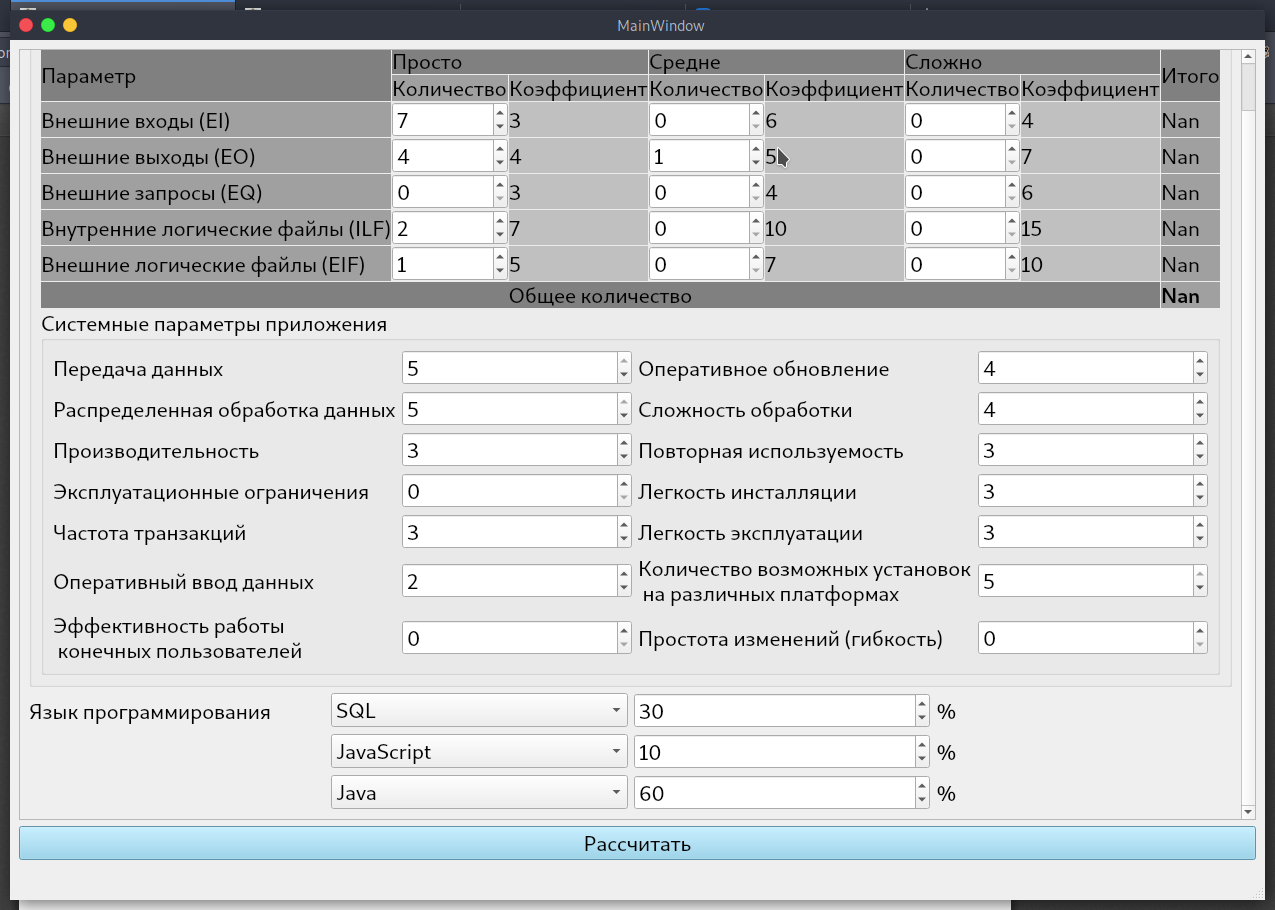
\includegraphics[width=16cm]{fp_set}}     \caption{Ввод данных для метода функциональных точек.}
    \label{fig:fp_set}
\end{figure}

\newpage
\begin{figure}[!h]
    \center{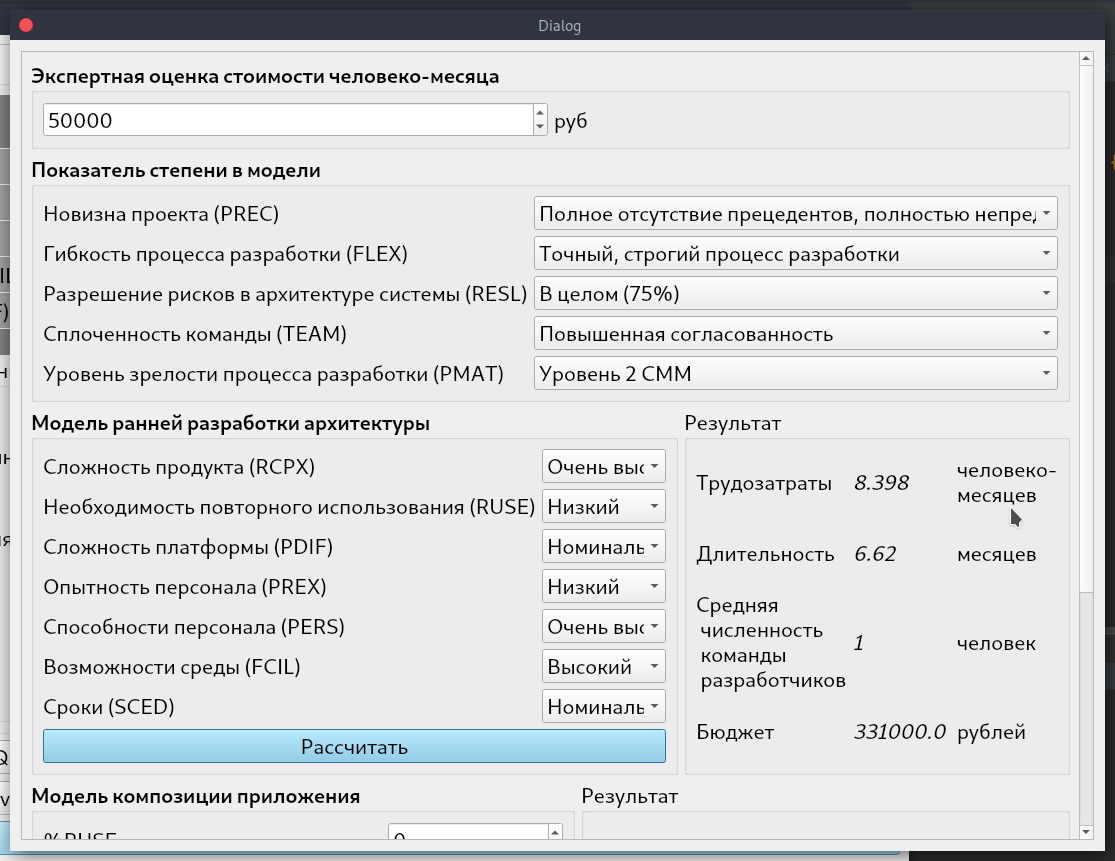
\includegraphics[width=16cm]{input1}}     \caption{Ввод данных для методики COCOMO2 (часть1).}
    \label{fig:input1}
\end{figure}

\newpage
\begin{figure}[!h]
    \center{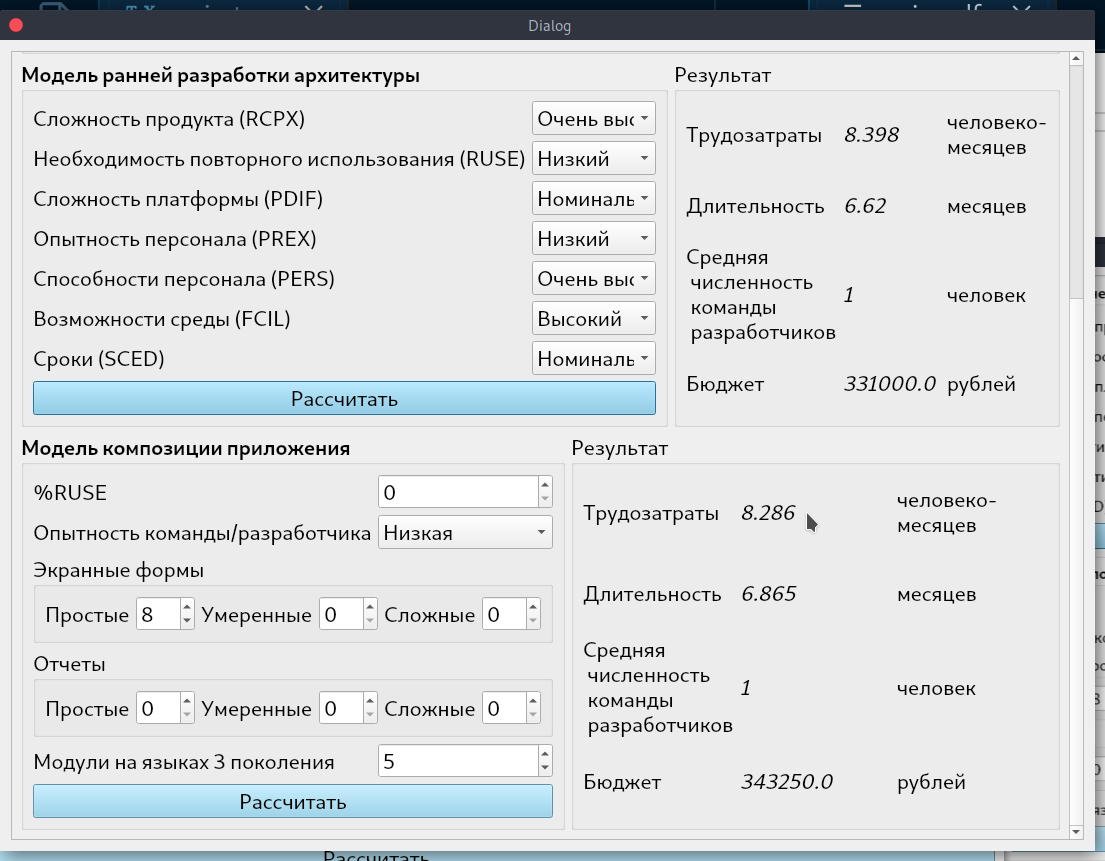
\includegraphics[width=16cm]{input2}}     \caption{Ввод данных для методики COCOMO2 (часть 2).}
    \label{fig:input2}
\end{figure}

\subsection*{Вывод}

Модель COCOMO2 позволяет более полно учитывать факторы, влияющих на экономические характеристики производства сложных программных продуктов, а также учитывать уникальные факторы для корректировки экономических характеристик, связанные со специфическим проектом и организацией.

COCOMO2 и метод функциональных точек предоставляет возможность оценить объем проекта если собственный опыт аналогичных проектов отсутствует, а экспертное мнение недоступно.

\end{document}
